In this section, we show empirical results of our algorithm for different transferring situations on two image benchmark datasets: Office and Caltech.
\subsection{Dataset \& Baseline methods}
Office contains 31 classes from 3 subsets (Amazon, Dslr and Webcam) and Caltech contains 256 classes. We select 13 shared classes from two datasets\footnote{13 classes include: backpack, bike, helmet, bottle, calculator, headphone, keyboard, laptop, monitor, mouse, mug, phone and projector}. The input features of all examples are extracted using AlexNet\cite{krizhevsky2012imagenet}.
%Because the two subsets Dslr and Webcam are relatively small and don't have data for testing, we only use them as the source domain.
\begin{table}[htbp]
	\centering
	\caption{Statistics of the datasets and subsets}
	\begin{tabular}{|c|c|c|c|c|}
		\hline
		Dataset&Subsets&\# classes &\# examples & \# features\\\hline
		\multirow{3}{*}{Office} & Amazon (A) &13&1173 & 4096\\
		
		& Dslr (D) &13&224 & 4096\\
		& Webcam (W) &13&369 & 4096\\
		\hline
		Caltech256&Caltech (C)&13&1582&4096\\
		\hline
	\end{tabular}%
	\label{tab:class_info}%
\end{table}%
We compare our algorithm EMTLe with two kinds of baselines. The first one is the methods without leveraging any source knowledge (no transfer baselines), including two methods. \textbf{No transfer:} SVMs trained only on target data. Any transfer algorithm that performs worse than it suffers from negative transfer. \textbf{Batch:} We combine the source and target data, assuming that we have full access to all data, to train the SVMs. The result of the Batch method is expected to outperform other methods under the HTL setting as it can access the source data. The second kind of baseline consists of two previous transfer methods in HTL, \textbf{MKTL\cite{jie2011multiclass}} and \textbf{Multi-KT\cite{tommasi2014learning}}. Similar to EMTLe, both of them use the LOOCV method to estimate the relatedness of the source model and target domain, but they use their convex objective function without the $\ell_2$ penalty terms. We use linear kernel for all methods in all our experiments.
\subsection{Transfer from Single Source Domain}
In this subsection, following the experiment protocol in \cite{jie2011multiclass,tommasi2014learning} for a fair comparison, we perform 12 groups of experiments under the setting of HTL. 
For each experiment, one of the 4 (sub)datasets is selected as the source, while another dataset is used as the target. We evaluate the performance of EMTLe when all source models are of the same type. As Multi-KT can only leverage knowledge when the source model is SVM, All source models are trained with linear SVMs.
The size of each target dataset is varied from 1 to 5 to see how EMTLe and other baselines behave under the extremely small dataset. We use a heuristic way to set the value of $\lambda$ in Eq. \eqref{eq:bo_high}:
\begin{equation}
\lambda = 2e^{err_{n}-err_{s}}
\end{equation}
where $err_{n}$ and $err_{s}$ denote the performance of ``No transfer'' and the source model on the training set.
We perform each experiment 10 times and report the average result in Figure \ref{fig:exp}. 
\begin{figure}[th]
\centering
\subfloat[C$\rightarrow$A]{
    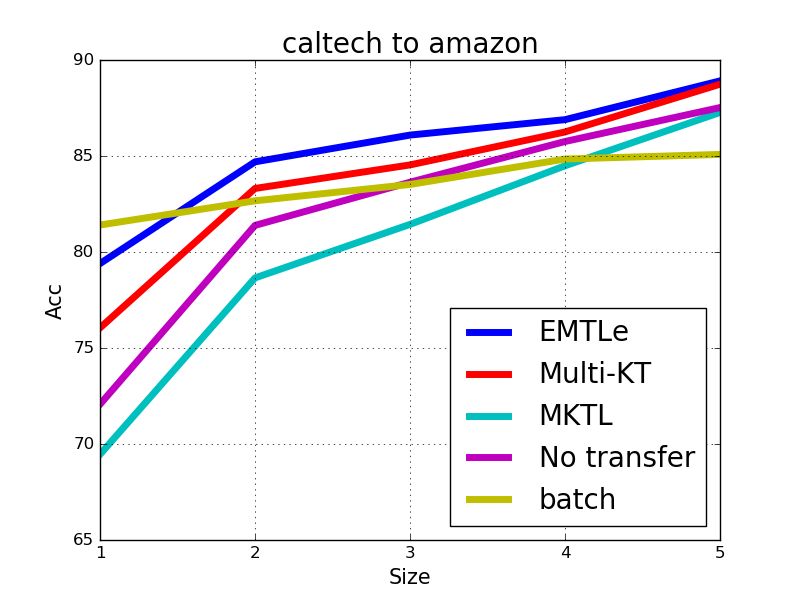
\includegraphics[width=0.30\textwidth]{pakdd/fig/caltechtoamazon.png}\label{a}
}
\subfloat[D$\rightarrow$A]{
    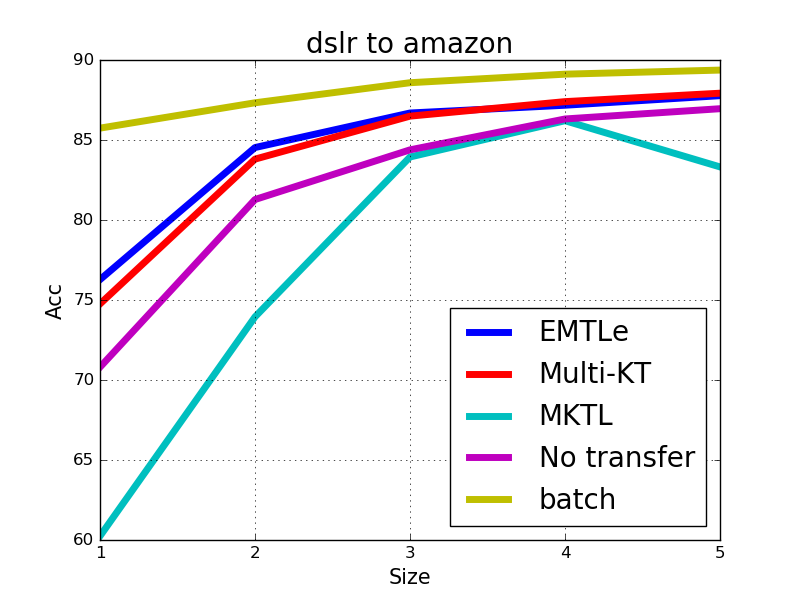
\includegraphics[width=0.30\textwidth]{pakdd/fig/dslrtoamazon.png}\label{b}
}
\subfloat[W$\rightarrow$A]{
	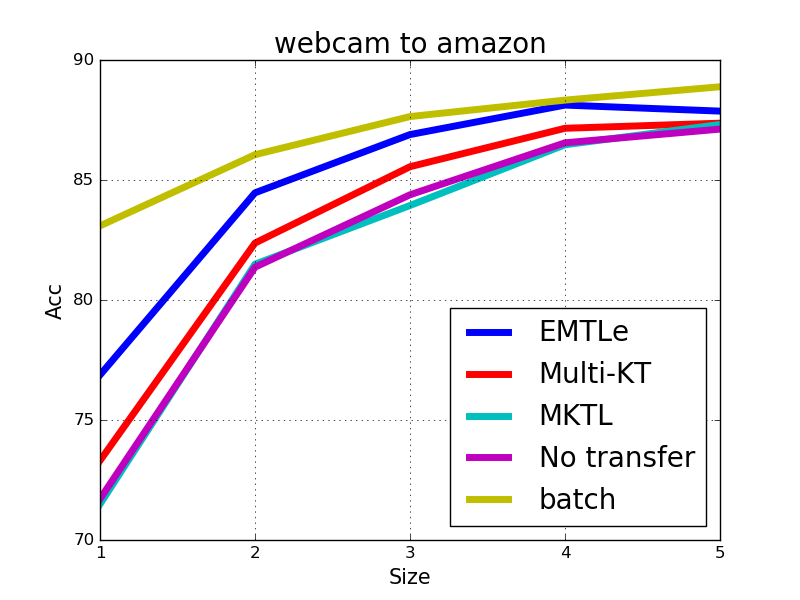
\includegraphics[width=0.30\textwidth]{pakdd/fig/webcamtoamazon.png}\label{c}
}\\
\subfloat[A$\rightarrow$C]{
	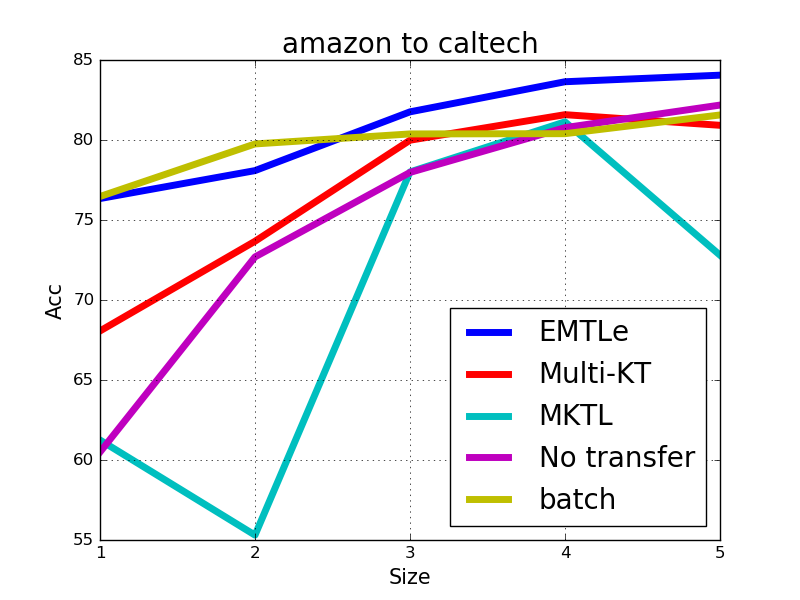
\includegraphics[width=0.30\textwidth]{pakdd/fig/amazontocaltech.png}\label{d}
}
\subfloat[D$\rightarrow$C]{
	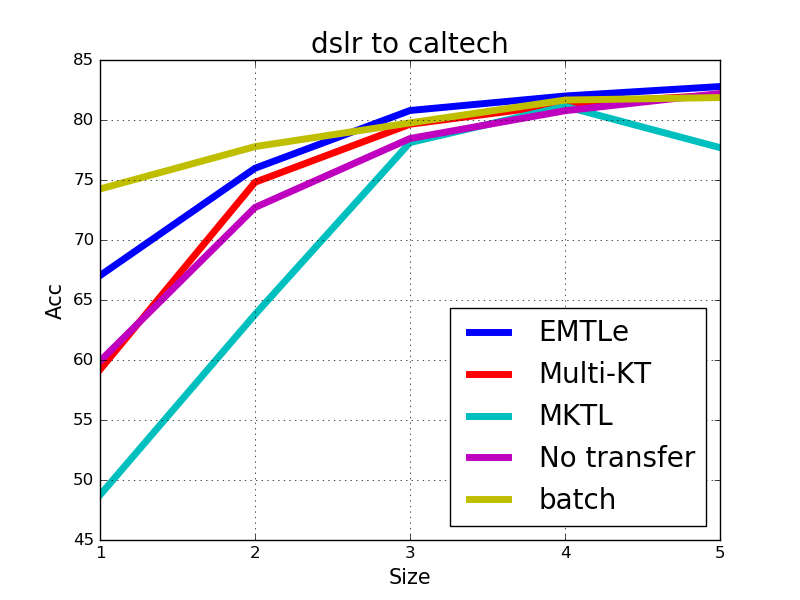
\includegraphics[width=0.30\textwidth]{pakdd/fig/dslrtocaltech.png}\label{e}
}
\subfloat[W$\rightarrow$C]{
	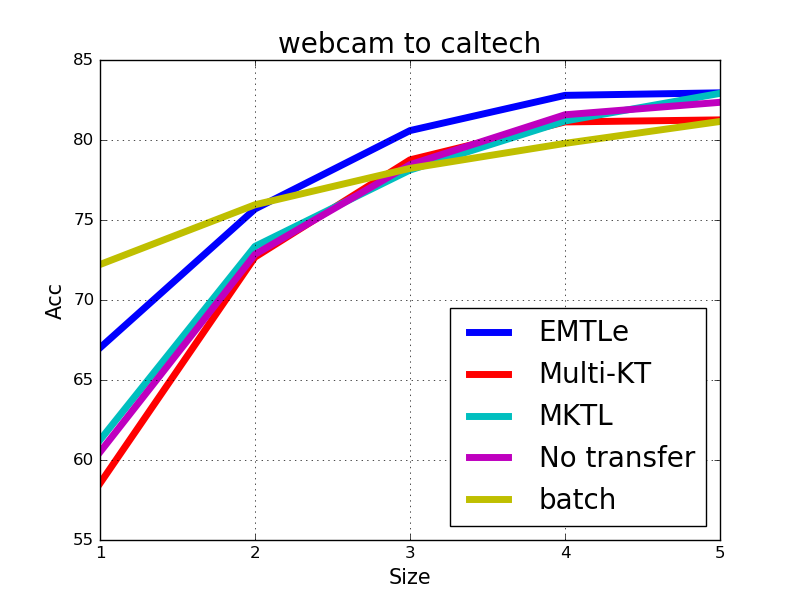
\includegraphics[width=0.30\textwidth]{pakdd/fig/webcamtocaltech.png}\label{f}
}\\
\subfloat[A$\rightarrow$D]{
	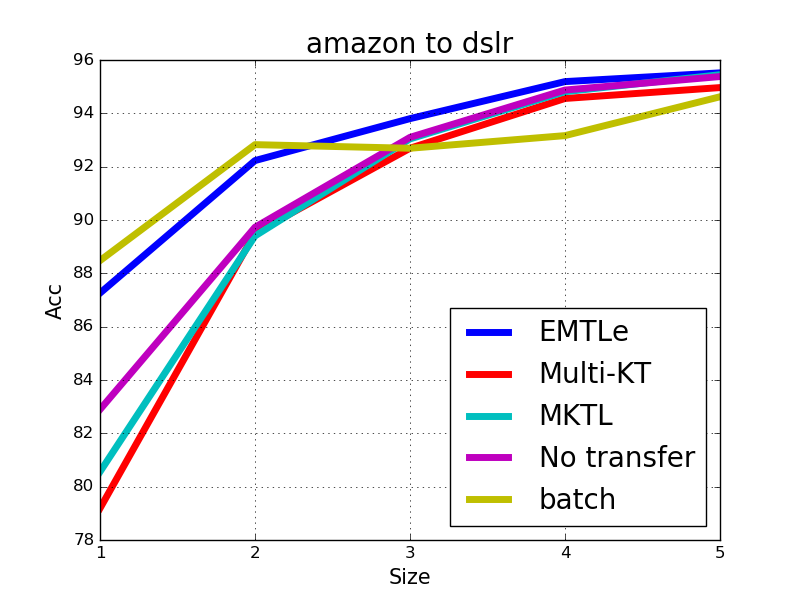
\includegraphics[width=0.30\textwidth]{pakdd/fig/amazontodslr.png}\label{g}
}
\subfloat[C$\rightarrow$D]{
	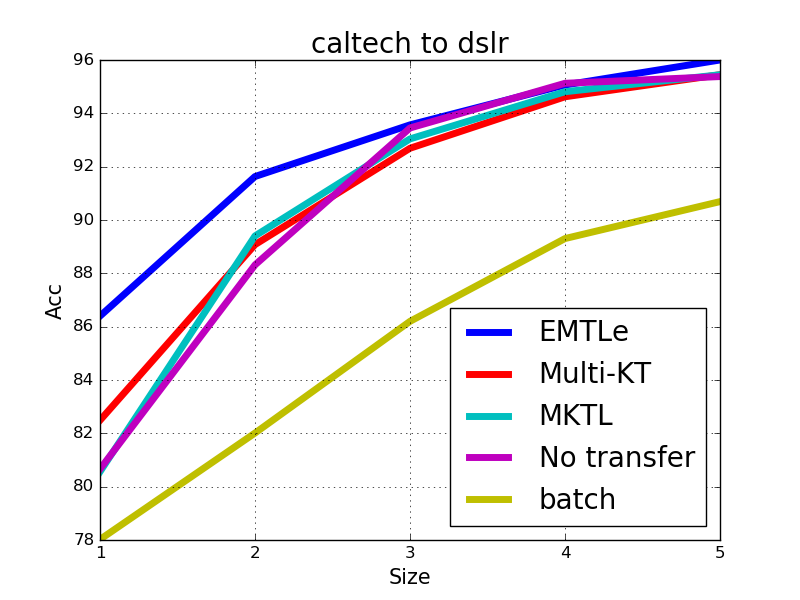
\includegraphics[width=0.30\textwidth]{pakdd/fig/caltechtodslr.png}\label{h}
}
\subfloat[W$\rightarrow$D]{
	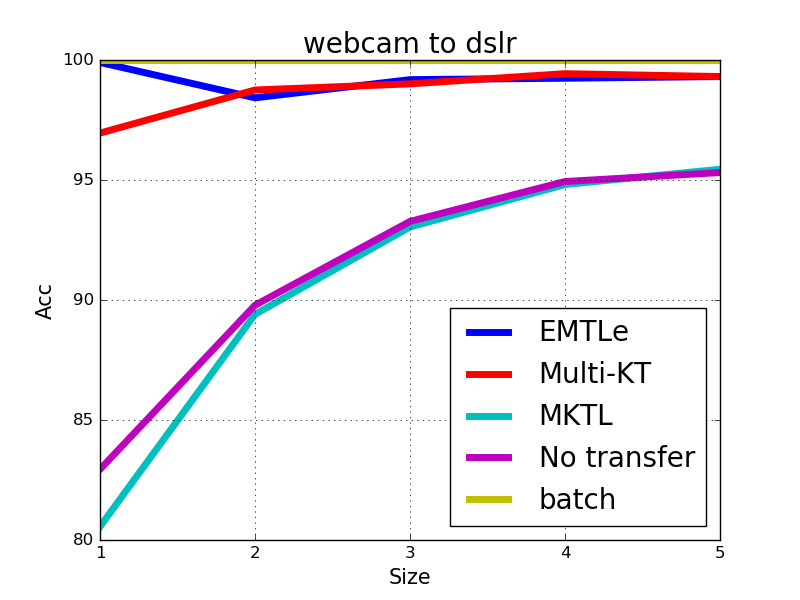
\includegraphics[width=0.30\textwidth]{pakdd/fig/webcamtodslr.png}\label{i}
}\\
\subfloat[A$\rightarrow$W]{
	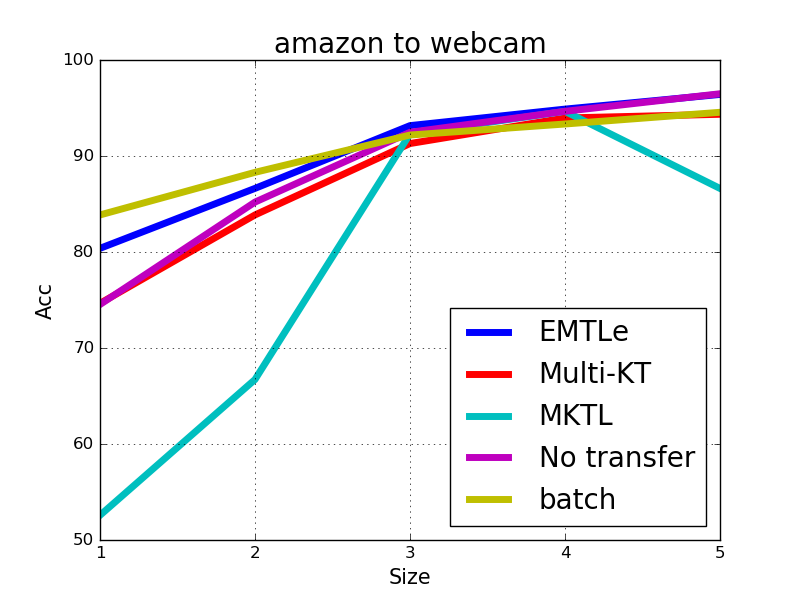
\includegraphics[width=0.30\textwidth]{pakdd/fig/amazontowebcam.png}\label{j}
}
\subfloat[C$\rightarrow$W]{
	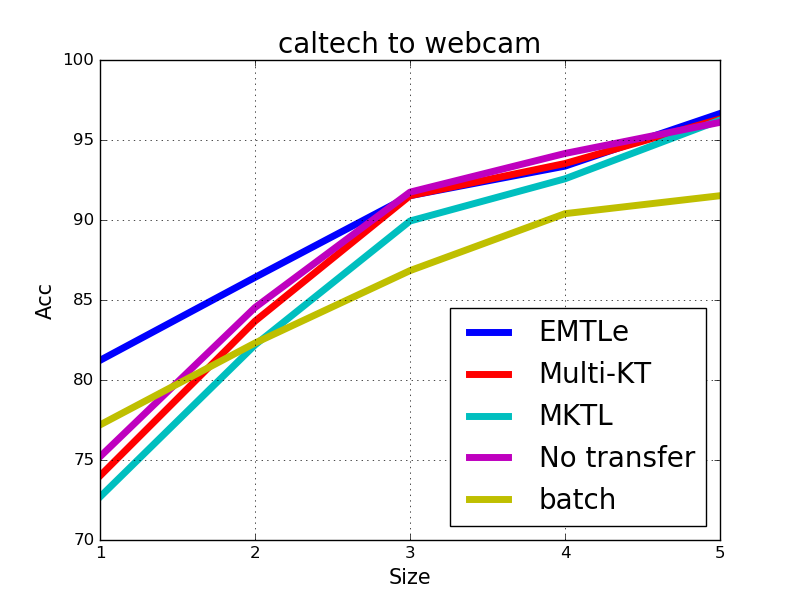
\includegraphics[width=0.30\textwidth]{pakdd/fig/caltechtowebcam.png}\label{k}
}
\subfloat[D$\rightarrow$W]{
	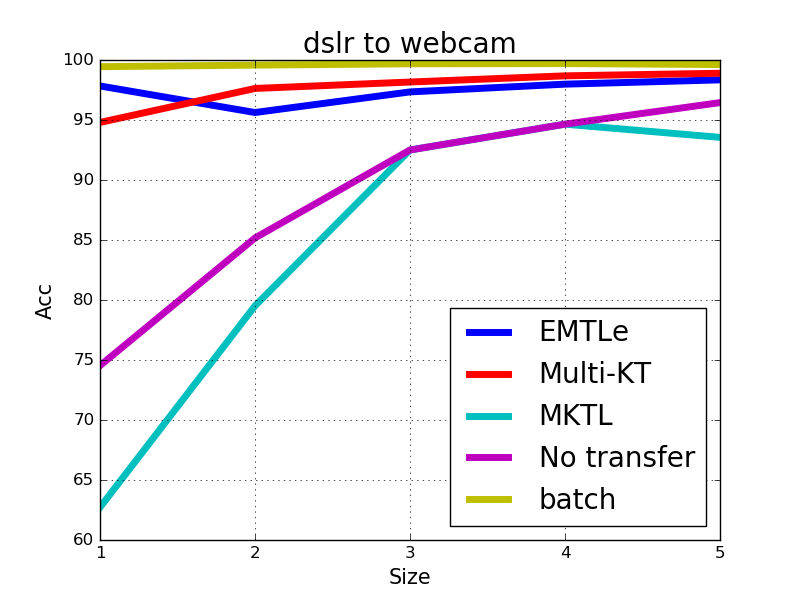
\includegraphics[width=0.30\textwidth]{pakdd/fig/dslrtowebcam.png}\label{l}
}
\caption{Recognition accuracy for HTL domain adaptation from a single source. 5 different sizes of target training sets are used in each group of experiments. A, D, W and C denote the 4 subsets in Table \ref{tab:class_info} respectively.}
\label{fig:exp}
\end{figure}

\textbf{Observation \& discussion:} EMTLe can significantly outperform other baselines especially with a small training set. %Moreover, in some groups of experiments, they even suffer from negative transfer on the small training set. 
As we have discussed above, when the training set is small, with the transfer parameter estimated by our $\ell_2$ penalty in our high-level objective functions, EMTLe has a strong generalization ability and performs better on the test data. As the training size increases, the variance of training data decreases and the affect of the $\ell_2$ penalty term become less significant. Therefore, EMTLe and the other two HTL baselines show similar performance. 
It is interesting to see that MKTL even falls into negative transfer even with 5 training examples per class in some experiments. We found that, MKTL is more sensitive to the variance of the training data. Its performance is not as stable as Multi-KT and EMTLe over the 10 experiments. Because MKTL needs to learn more hyperparameters than Multi-KT and EMTLe, even though the training size increases, it may not be able to obtain a good model. 
In some experiments, we can see that EMTLe can even outperform the Batch method which can access more information and is expected to outperform the other methods under the setting of HTL.

\subsection{Transfer from Multiple Source Domains}
As we mentioned, EMTLe can exploit knowledge from different types of source classifiers which could greatly extend our choice of the source domain under the HTL setting. In this subsection, we show that EMTLe can successfully transfer the knowledge from two different types of source classifiers. Meanwhile, MKTL and ``No Transfer" are used as our baseline. 

In this experiment, we assume that there is no single source domain that can cover all 13 classes in our target domain and we have to select source models from different source domains. Specifically, the 13 classes are selected from two different domains separately (6 from DSLR and 7 from Webcam) according to Table \ref{tab:class_gen}. Similar to our previous experiment configurations, we only use Caltech and Amazon as the target domains. We show the experiment results in Figure \ref{fig:exp2}.
% Table generated by Excel2LaTeX from sheet 'Sheet1'
\begin{table}[htbp]
	\centering
	\caption{The selected classes of the two source domains and the classifier type of the source model.}
	\begin{tabular}{|c|c|c|}
		\hline
		& class & classifier\\
		\hline
		DSRL& monitor,bike, helmet,calcu,headphone,projector & Logistic\\\hline
		Webcam&keyboard,mouse,phone,backpack,mug,bottle,laptop&SVMs\\ \hline
		
	\end{tabular}%
	\label{tab:class_gen}%
\end{table}%
\begin{figure}[h]
	\centering
	\subfloat[D+W $\rightarrow$ A]{
		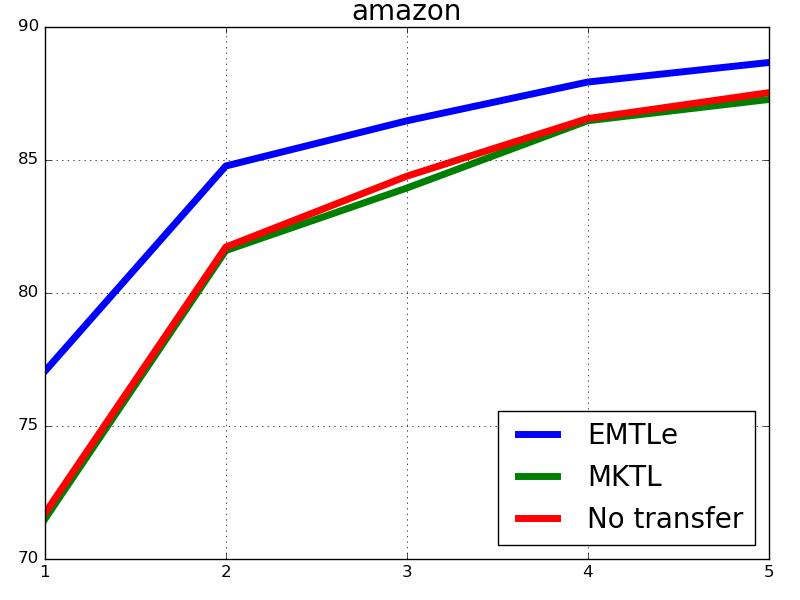
\includegraphics[width=0.5\textwidth]{pakdd/fig/multi_amazon.png}\label{a2}
	}
	\subfloat[D+W $\rightarrow$ C]{
		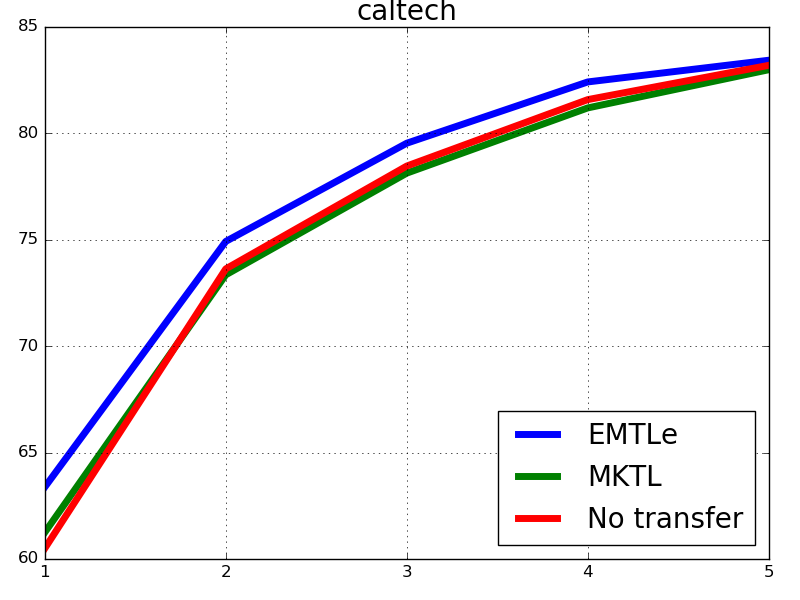
\includegraphics[width=0.5\textwidth]{pakdd/fig/multi_caltech.png}\label{b2}
	}\\
	\caption{Recognition Accuracy for Multi-Model \& Multi-Source experiment on two target datasets. }
	\label{fig:exp2}
\end{figure}

\textbf{Observation \& discussion:} In our multi-source scenario, it is more difficult to leverage the knowledge from the source models as the models are trained from different domains separately. From the results we can see that, EMTLe can still exploit the knowledge from the source models despite the types of the source classifiers while MKTL can hardly leverage the source knowledge. EMTLe uses a simple way to leverage the source models and BO can help us better estimate the transfer parameter. However, MKTL uses a sophisticated feature augmentation and has more hyperparameters to estimate. Without sufficient training data, it is difficult for MKTL to measure the importance of each source model and exploit the knowledge from the models.




